\documentclass[a4paper,12pt]{article}

\usepackage[T1]{fontenc}
\usepackage[utf8]{inputenc}
\usepackage[french]{babel}
\usepackage{geometry}
\usepackage{fancyhdr}
\usepackage{titlesec}
\usepackage{parskip}
\usepackage{booktabs}
\usepackage{tabularx}
\usepackage{listings}
\usepackage{xcolor}
\usepackage{hyperref}
\usepackage{enumitem}
\usepackage{lmodern}
\usepackage{colortbl}
\usepackage{float}
\usepackage{graphicx}

\geometry{top=3cm, bottom=3cm, left=3cm, right=3cm}

% Couleurs discrètes
\definecolor{codebg}{HTML}{F5F5F5}
\definecolor{codefg}{HTML}{333333}
\definecolor{gris}{HTML}{666666}

% Style de code sobre
\lstdefinestyle{code}{
    backgroundcolor=\color{codebg},
    basicstyle=\ttfamily\small\color{codefg},
    breaklines=true,
    frame=single,
    rulecolor=\color{lightgray},
    xleftmargin=8pt,
    xrightmargin=8pt,
    aboveskip=6pt,
    belowskip=6pt,
}
\lstset{style=code}

% Titres sobres
\titleformat{\section}{\large\bfseries}{}{0em}{}[\vspace{-0.3em}\rule{\textwidth}{0.4pt}]
\titleformat{\subsection}{\normalsize\bfseries}{}{0em}{}

% En-tête / pied de page
\pagestyle{fancy}
\fancyhf{}
\fancyhead[L]{\small\textit{Rapport de pentest — Red Team}}
\fancyhead[R]{\small\textit{ECE Paris — 2025/2026}}
\fancyfoot[C]{\small\thepage}
\renewcommand{\headrulewidth}{0.3pt}

\hypersetup{colorlinks=true, linkcolor=black, urlcolor=black}

% ══════════════════════════════════════════════════════════════════════════════
\begin{document}

% ── Page de garde ─────────────────────────────────────────────────────────────
\begin{titlepage}
\centering
\vspace*{4cm}

{\Large\bfseries Rapport de test d'intrusion}\\[0.4cm]
{\large Projet final — Cyber Challenge}\\[0.2cm]
{\normalsize\color{gris} Red Team}

\vspace{3cm}

\begin{tabular}{rl}
    Auteur      & Romain LIGNERES \\
    Filière     & Cyber \\
    Binôme      & Arthur LAUZANNE - Blue team \\
    École       & ECE Paris \\
    Année       & 2025-2026 \\
    Date        & \today \\
\end{tabular}

\vfill
{\small\color{gris} Cours : Sécurité des Systèmes d'Information — M. Badr Tajini}
\end{titlepage}

% ── Table des matières ────────────────────────────────────────────────────────
\tableofcontents
\newpage

% ══════════════════════════════════════════════════════════════════════════════
\section{Introduction}

Ce rapport documente les tests d'intrusion menés sur la façade Moodle développée par la Blue Team
dans le cadre du projet final du cours Sécurité des SI. L'objectif était d'identifier et d'exploiter
des vulnérabilités web afin de compromettre l'application, puis de formuler des recommandations
concrètes pour y remédier.

Les tests ont été réalisés dans un cadre pédagogique contrôlé. L'application cible tourne en local
et a été développée volontairement avec des failles pour cet exercice.

% ══════════════════════════════════════════════════════════════════════════════
\section{Périmètre}

\begin{tabular}{ll}
    \toprule
    \textbf{Élément}      & \textbf{Détail} \\
    \midrule
    Application           & Façade Moodle simplifiée (Blue Team) \\
    URL                   & \texttt{http://localhost:3000} \\
    Technologies          & Node.js, Express.js, SQLite \\
    Pages testées         & \texttt{/login}, \texttt{/calendar}, ... \\
    \bottomrule
\end{tabular}

% ══════════════════════════════════════════════════════════════════════════════
\section{Méthodologie}

Les tests ont suivi trois étapes classiques en pentest applicatif :

\begin{enumerate}
    \item \textbf{Reconnaissance} — analyse du comportement de l'application via le navigateur,
    inspection du code source côté client, identification des points d'entrée.

    \item \textbf{Exploitation} — envoi de payloads manuels sur les champs identifiés,
    observation des réponses du serveur.

    \item \textbf{Documentation} — capture des preuves, rédaction du présent rapport.
\end{enumerate}

\newpage

% ══════════════════════════════════════════════════════════════════════════════
\section{Vulnérabilité 1 — Injection SQL}

\subsection{Localisation}

Route \texttt{POST /login} — traitement du formulaire de connexion.

\subsection{Description}

Lors de mes tests sur le formulaire de connexion, j'ai d'abord tenté d'insérer une apostrophe simple dans le champ username. Le serveur a retourné une erreur de base de données, ce qui m'a confirmé que mon entrée était directement interprétée dans la requête SQL sans aucun filtrage.
J'ai ensuite utilisé un payload classique d'injection SQL pour contourner l'authentification.

\subsection{Exploitation}

Dans le champ \textit{Nom d'utilisateur}, j'ai saisi le payload suivant :

\begin{lstlisting}
' OR '1'='1'--
\end{lstlisting}

Avec n'importe quelle valeur dans le champ mot de passe, la requête exécutée devient :

\begin{lstlisting}
SELECT * 
FROM users 
WHERE username = '' OR '1'='1'--' 
AND password = ''
\end{lstlisting}

La condition \texttt{'1'='1'} étant toujours vraie, le serveur retourne le premier utilisateur
de la base et accorde l'accès sans vérification du mot de passe.

\subsection{Preuve}

\begin{figure}[H]
    \centering
    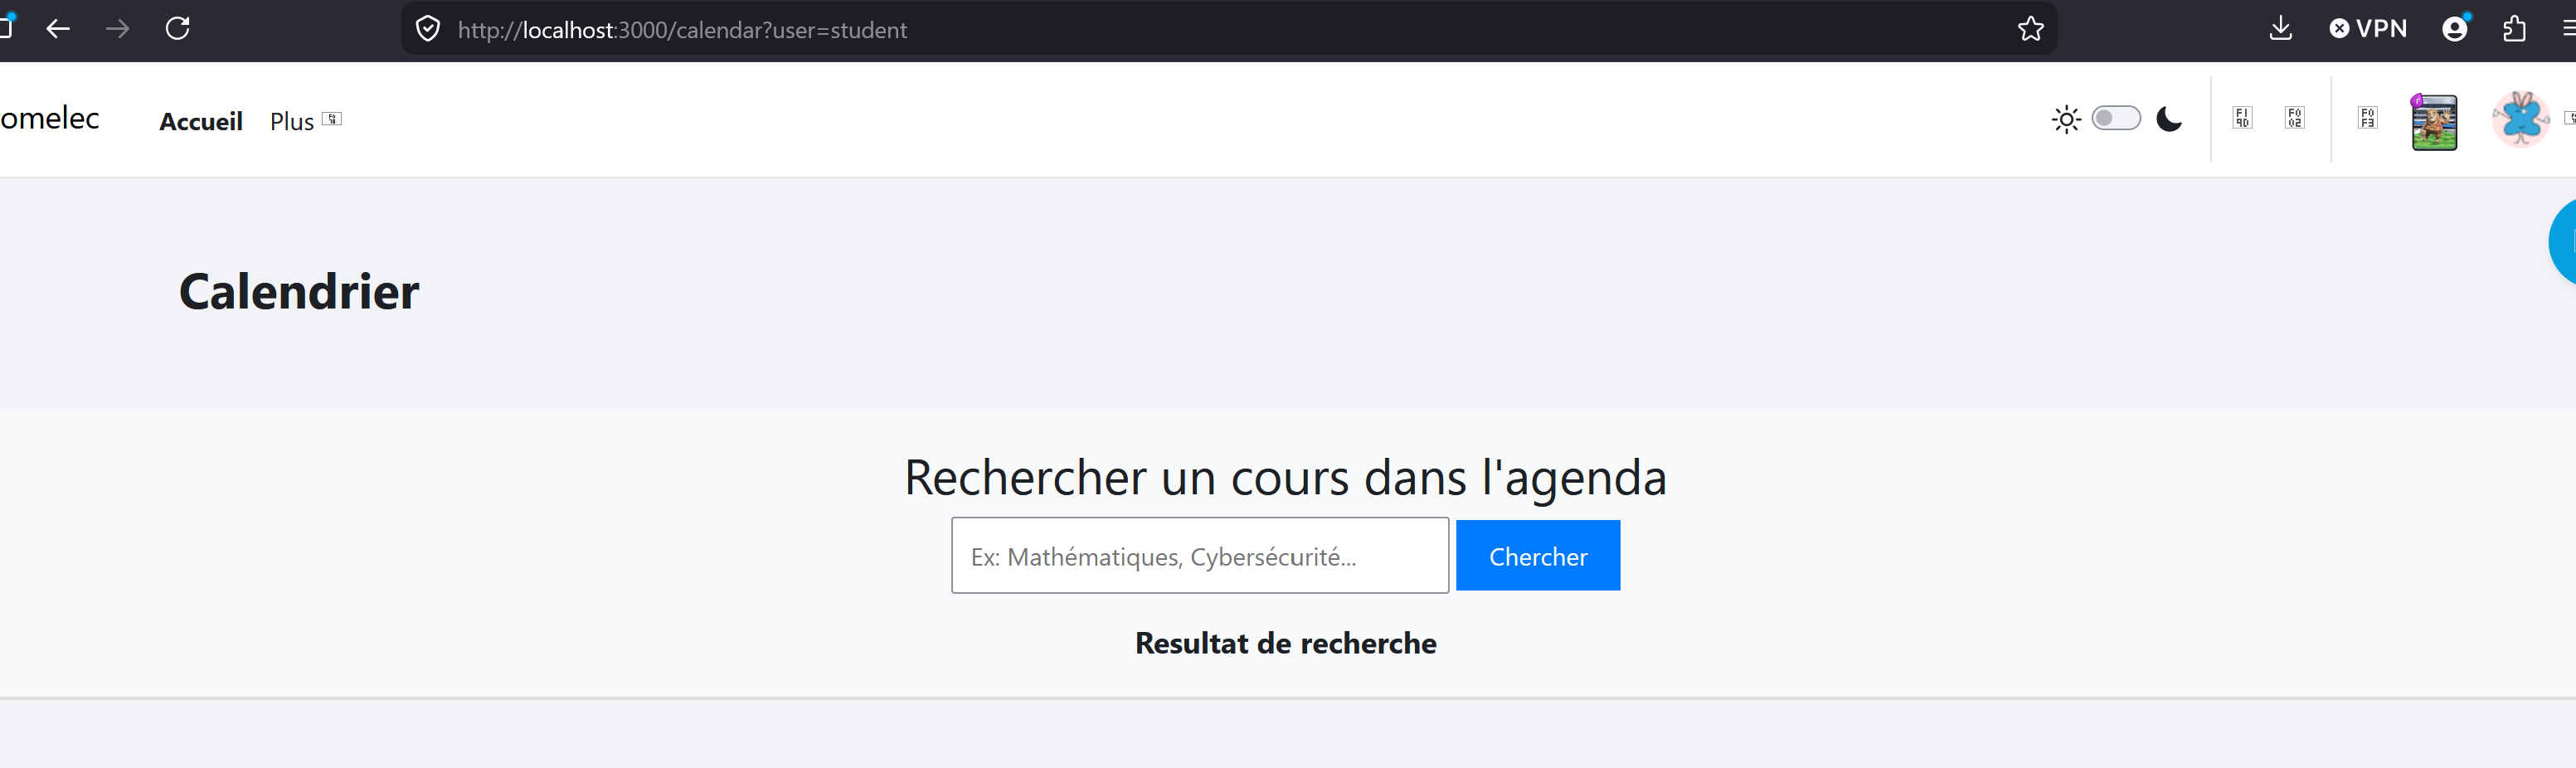
\includegraphics[width=0.9\linewidth]{pics/p1_ssiv1.png}
    \caption{Preuve de connexion sans connaître le mdp}
    \label{fig:placeholder}
\end{figure}


\subsection{Impact}

Contournement total de l'authentification. Dans un contexte réel, un attaquant pourrait accéder
à l'ensemble des fonctionnalités réservées aux utilisateurs connectés.

\subsection{Recommandation}

Utiliser des requêtes préparées avec paramètres liés :

\begin{lstlisting}
db.get(
  "SELECT * FROM users WHERE username = ? AND password = ?",
  [username, password],
  callback
);
\end{lstlisting}

\newpage

% ══════════════════════════════════════════════════════════════════════════════
\section{Vulnérabilité 2 — XSS réfléchi}

\subsection{Localisation}

Route \texttt{GET /calendar} — paramètre d'URL \texttt{recherche}.

\subsection{Description}

En testant la barre de recherche, j'ai remarqué que ce que je tape apparaît directement dans la page et dans l'URL. J'ai alors testé si le site filtrait les balises HTML en injectant une balise <script>. Le navigateur a exécuté le code, confirmant la faille.


\subsection{Exploitation}

En naviguant vers l'URL suivante une fois connecté :

\begin{lstlisting}
http://localhost:3000/calendar?recherche=
  <script>alert('XSS')</script>
\end{lstlisting}

Ce qui s'est passé.
Une popup JavaScript s'est affichée avec le texte "XSS", prouvant que le code a été exécuté par le navigateur.
\subsection{Preuve}

\begin{figure}[H]
    \centering
    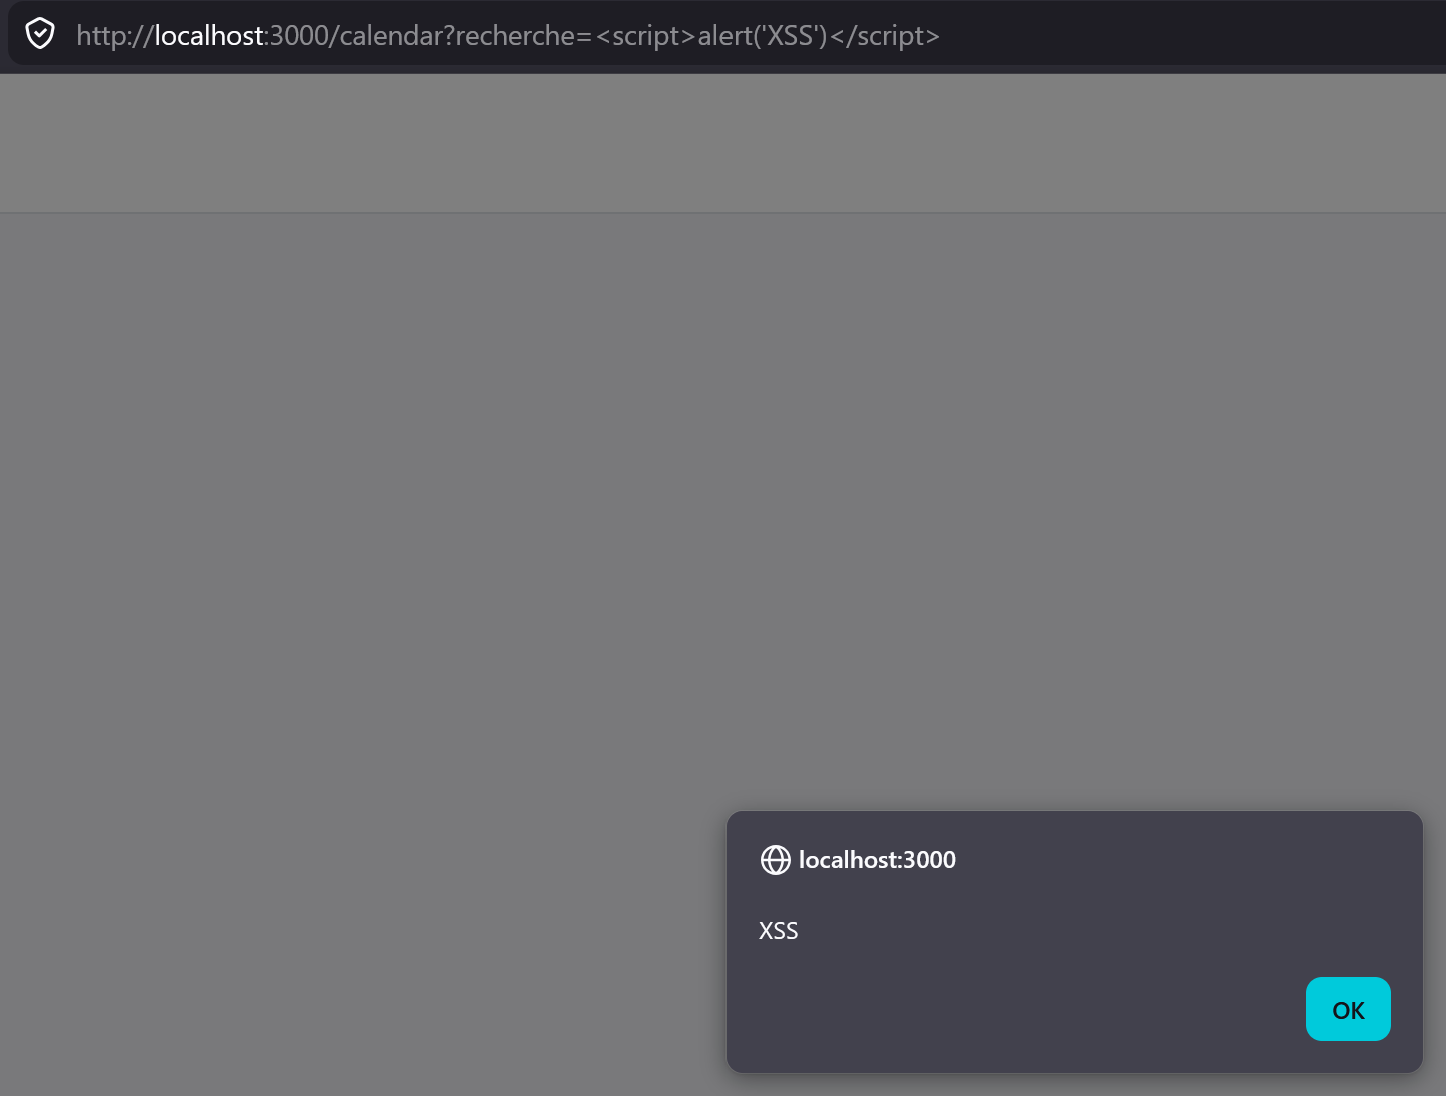
\includegraphics[width=0.8\linewidth]{pics/p2.png}
    \caption{Preuve d'injection de code malveillant}
    \label{fig:placeholder}
\end{figure}

\subsection{Impact}

Dans un contexte réel, un attaquant pourrait remplacer le alert par du code qui vole le cookie de session d'un utilisateur et se connecter à sa place sans connaître son mot de passe.

\subsection{Recommandation}

Échapper les caractères spéciaux avant toute insertion dans le HTML :

\begin{lstlisting}
const safe = motRecherche
  .replace(/&/g,  '&amp;')
  .replace(/</g,  '&lt;')
  .replace(/>/g,  '&gt;')
  .replace(/"/g,  '&quot;');
\end{lstlisting}

\newpage

% ══════════════════════════════════════════════════════════════════════════════
\section{Vulnérabilité 3 — XSS stocké}

\subsection{Localisation}

Route \texttt{GET /calendar?user=student}

\subsection{Description}

Lorsque j'ai voulu ajouter un commentaire en bas de page, je me suis rendu compte que je pouvais injecter du code avec des balises. Les balises HTML ne sont pas filtrées, ce qui permet d'injecter du code malveillant.


\subsection{Exploitation}

En naviguant vers l'URL suivante une fois connecté :

\begin{lstlisting}
  <b>teste</b>
\end{lstlisting}

Ce qui s'est passé.
J'ai pu afficher le mot "test" en gras grâce au balise html ce qui prouve la défaillance du système.
\subsection{Preuve}

\begin{figure}[H]
    \centering
    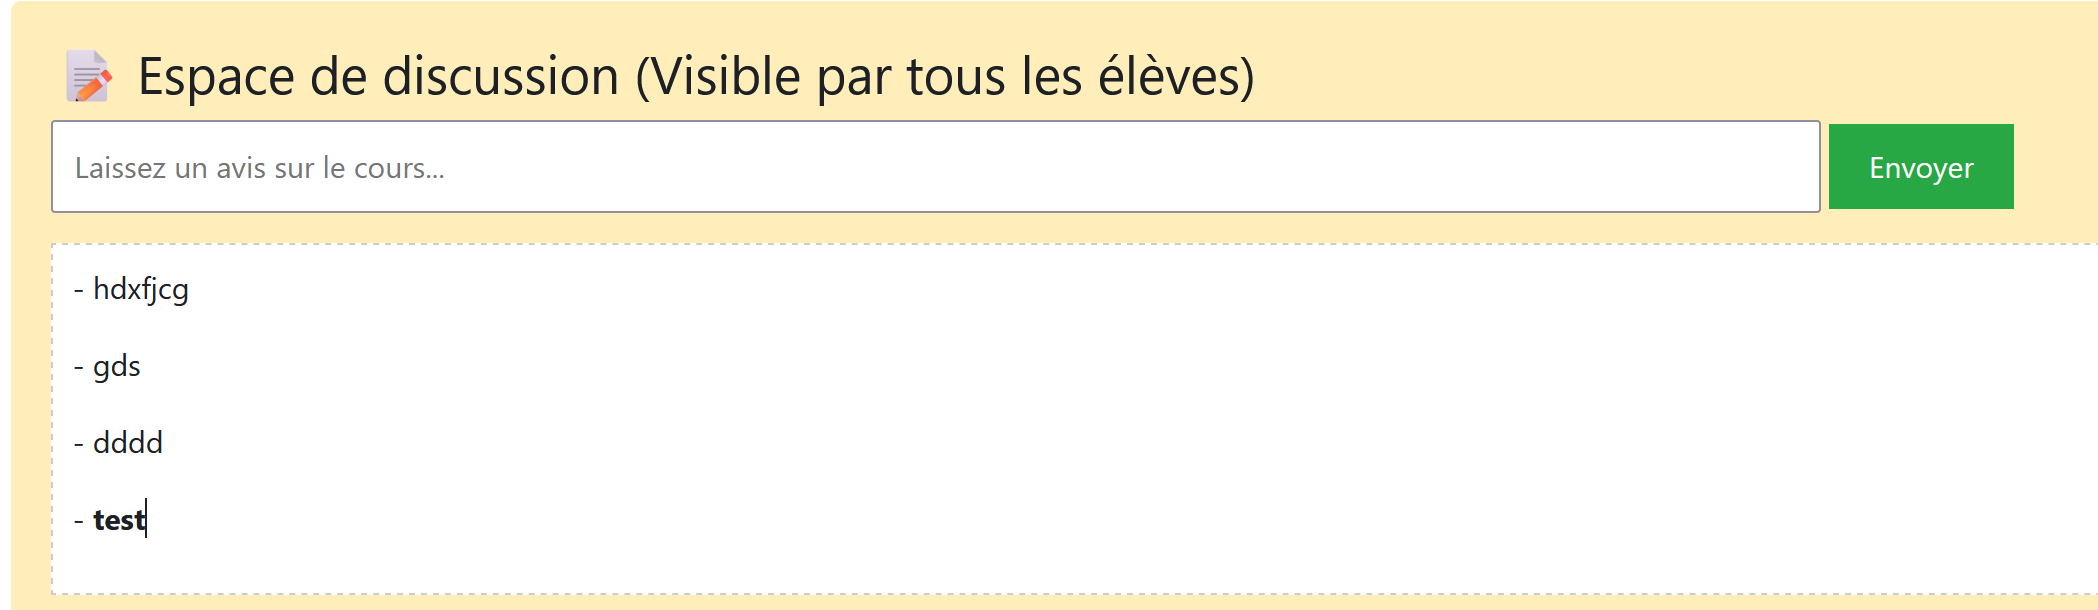
\includegraphics[width=0.8\linewidth]{pics/p3.png}
    \caption{Preuve d'injection de code malveillant dans l'espace de commentaire}
    \label{fig:placeholder}
\end{figure}

\subsection{Impact}

Tout code HTML inséré dans les commentaires est sauvegardé en base de données et réaffiché à tous les visiteurs sans nettoyage. Contrairement au XSS réfléchi qui ne touche qu'une personne via un lien piégé, ici le payload est permanent et s'exécute automatiquement pour chaque utilisateur qui charge la page. Dans un contexte réel avec des protections navigateur moins strictes, un attaquant pourrait voler les sessions de tous les utilisateurs connectés en une seule injection
\subsection{Recommandation}

Nettoyer toutes les données utilisateur avant de les stocker en base de données et avant de les afficher. En Node.js on peut utiliser la librairie DOMPurify ou simplement échapper les caractères HTML dangereux comme <, >, " avant l'insertion


\newpage
% ══════════════════════════════════════════════════════════════════════════════
\section{Vulnérabilité 4 — IDOR (Insecure Direct Object Reference)}

\subsection{Localisation}

Route \texttt{GET /calendar?user=student}

\subsection{Description}
J'ai remarqué que l'url de connexion pour un élève et de la forme /calendar?user=student, j'ai donc tenté de remplacer student par admin et je me suis retrouvé connecter en tant qu'admin.



\subsection{Exploitation}
Je me suis connecté via cette URL : /calendar?user=admin

\subsection{Preuve}

\begin{figure}[H]
    \centering
    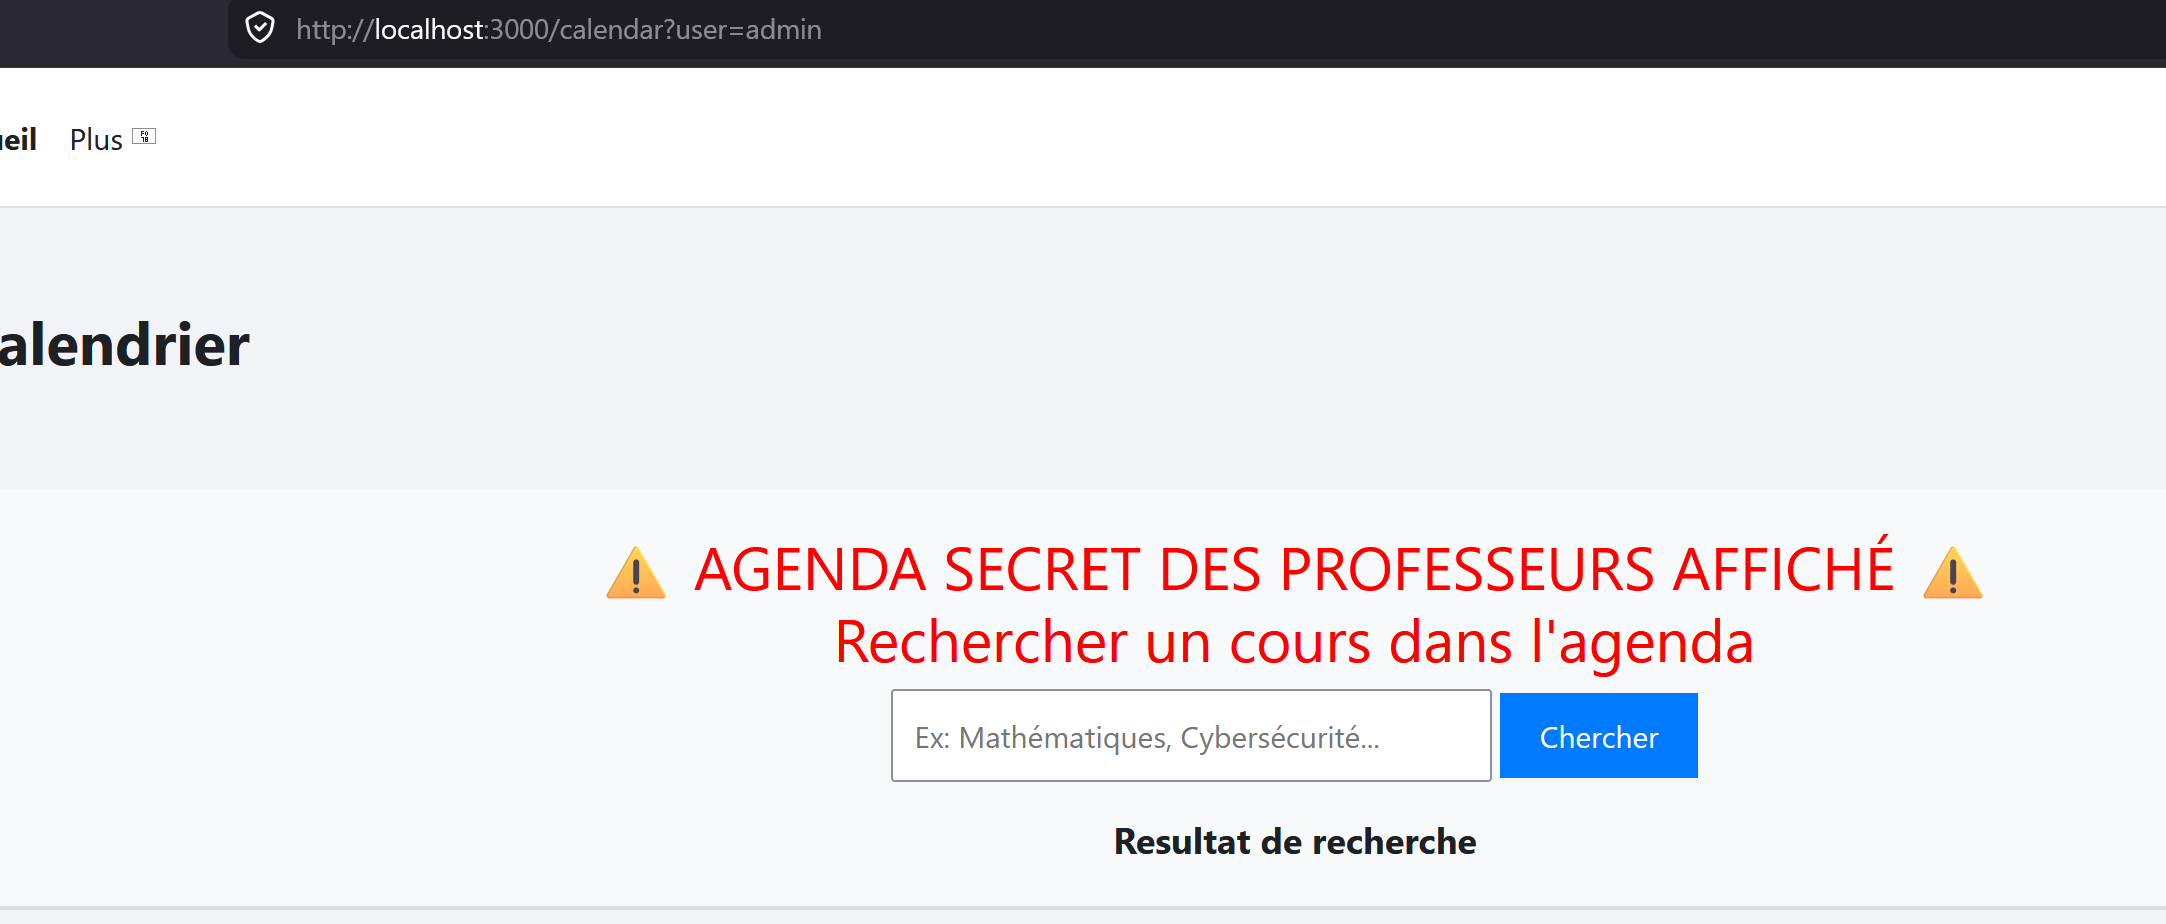
\includegraphics[width=0.8\linewidth]{pics/p4.png}
    \caption{Preuve de connexion à la page admin}
    \label{fig:placeholder}
\end{figure}

\subsection{Impact}
Je me suis retrouvé connecté à la page admin sans connaître le mot de passe. Un hacker peut donc récuperer toutes les infos ou les modifier sur cette page.

\subsection{Recommandation}
La correction de cette faille se fait côte serveur en vérifiant les rôles via un systèmes de session.

\newpage
% ══════════════════════════════════════════════════════════════════════════════
\section{Vulnérabilité 5 — Path Traversal}

\subsection{Localisation}

Route \texttt{GET /download?}

\subsection{Description}
J'ai remarqué que l'url pouvait être modifié sans vérification.
Le changement de l'URL permet de télécharger des nimporte quels fichiers du repo.


\subsection{Exploitation}
J'ai téléchagé le code du server.js via cet URL : /download?file=server.js

\subsection{Preuve}

\begin{figure}[H]
    \centering
    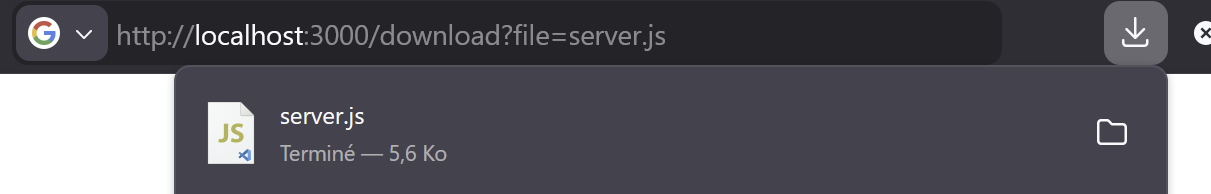
\includegraphics[width=0.8\linewidth]{pics/p5.png}
    \caption{Preuve de téléchargement du fichier server.js via la route /download}
    \label{fig:placeholder}
\end{figure}

\subsection{Impact}
Le télechargement s'est éffectué donc j'ai accès à tout le code ou fichier que je veux. Plus aucune informations n'est confidentielle avce cette faille.

\subsection{Recommandation}
Le serveur doit vérifier que le fichier demandé se trouve bien dans le dossier autorisé et refuser tout chemin contenant .. ou des références à des fichiers sensibles.
\newpage
% ══════════════════════════════════════════════════════════════════════════════
\section{Vulnérabilité 6 — Broken Access Control}

\subsection{Localisation}

Route \texttt{GET /admin}

\subsection{Description}
J'ai modifié l'URL et me suis directement connecté sur une page admin qui contient des infos sensibles.


\subsection{Exploitation}
La page /admin est accessible sans aucune vérification d'authentification. N'importe qui connaissant l'URL peut y accéder directement

\subsection{Preuve}

\begin{figure}[H]
    \centering
    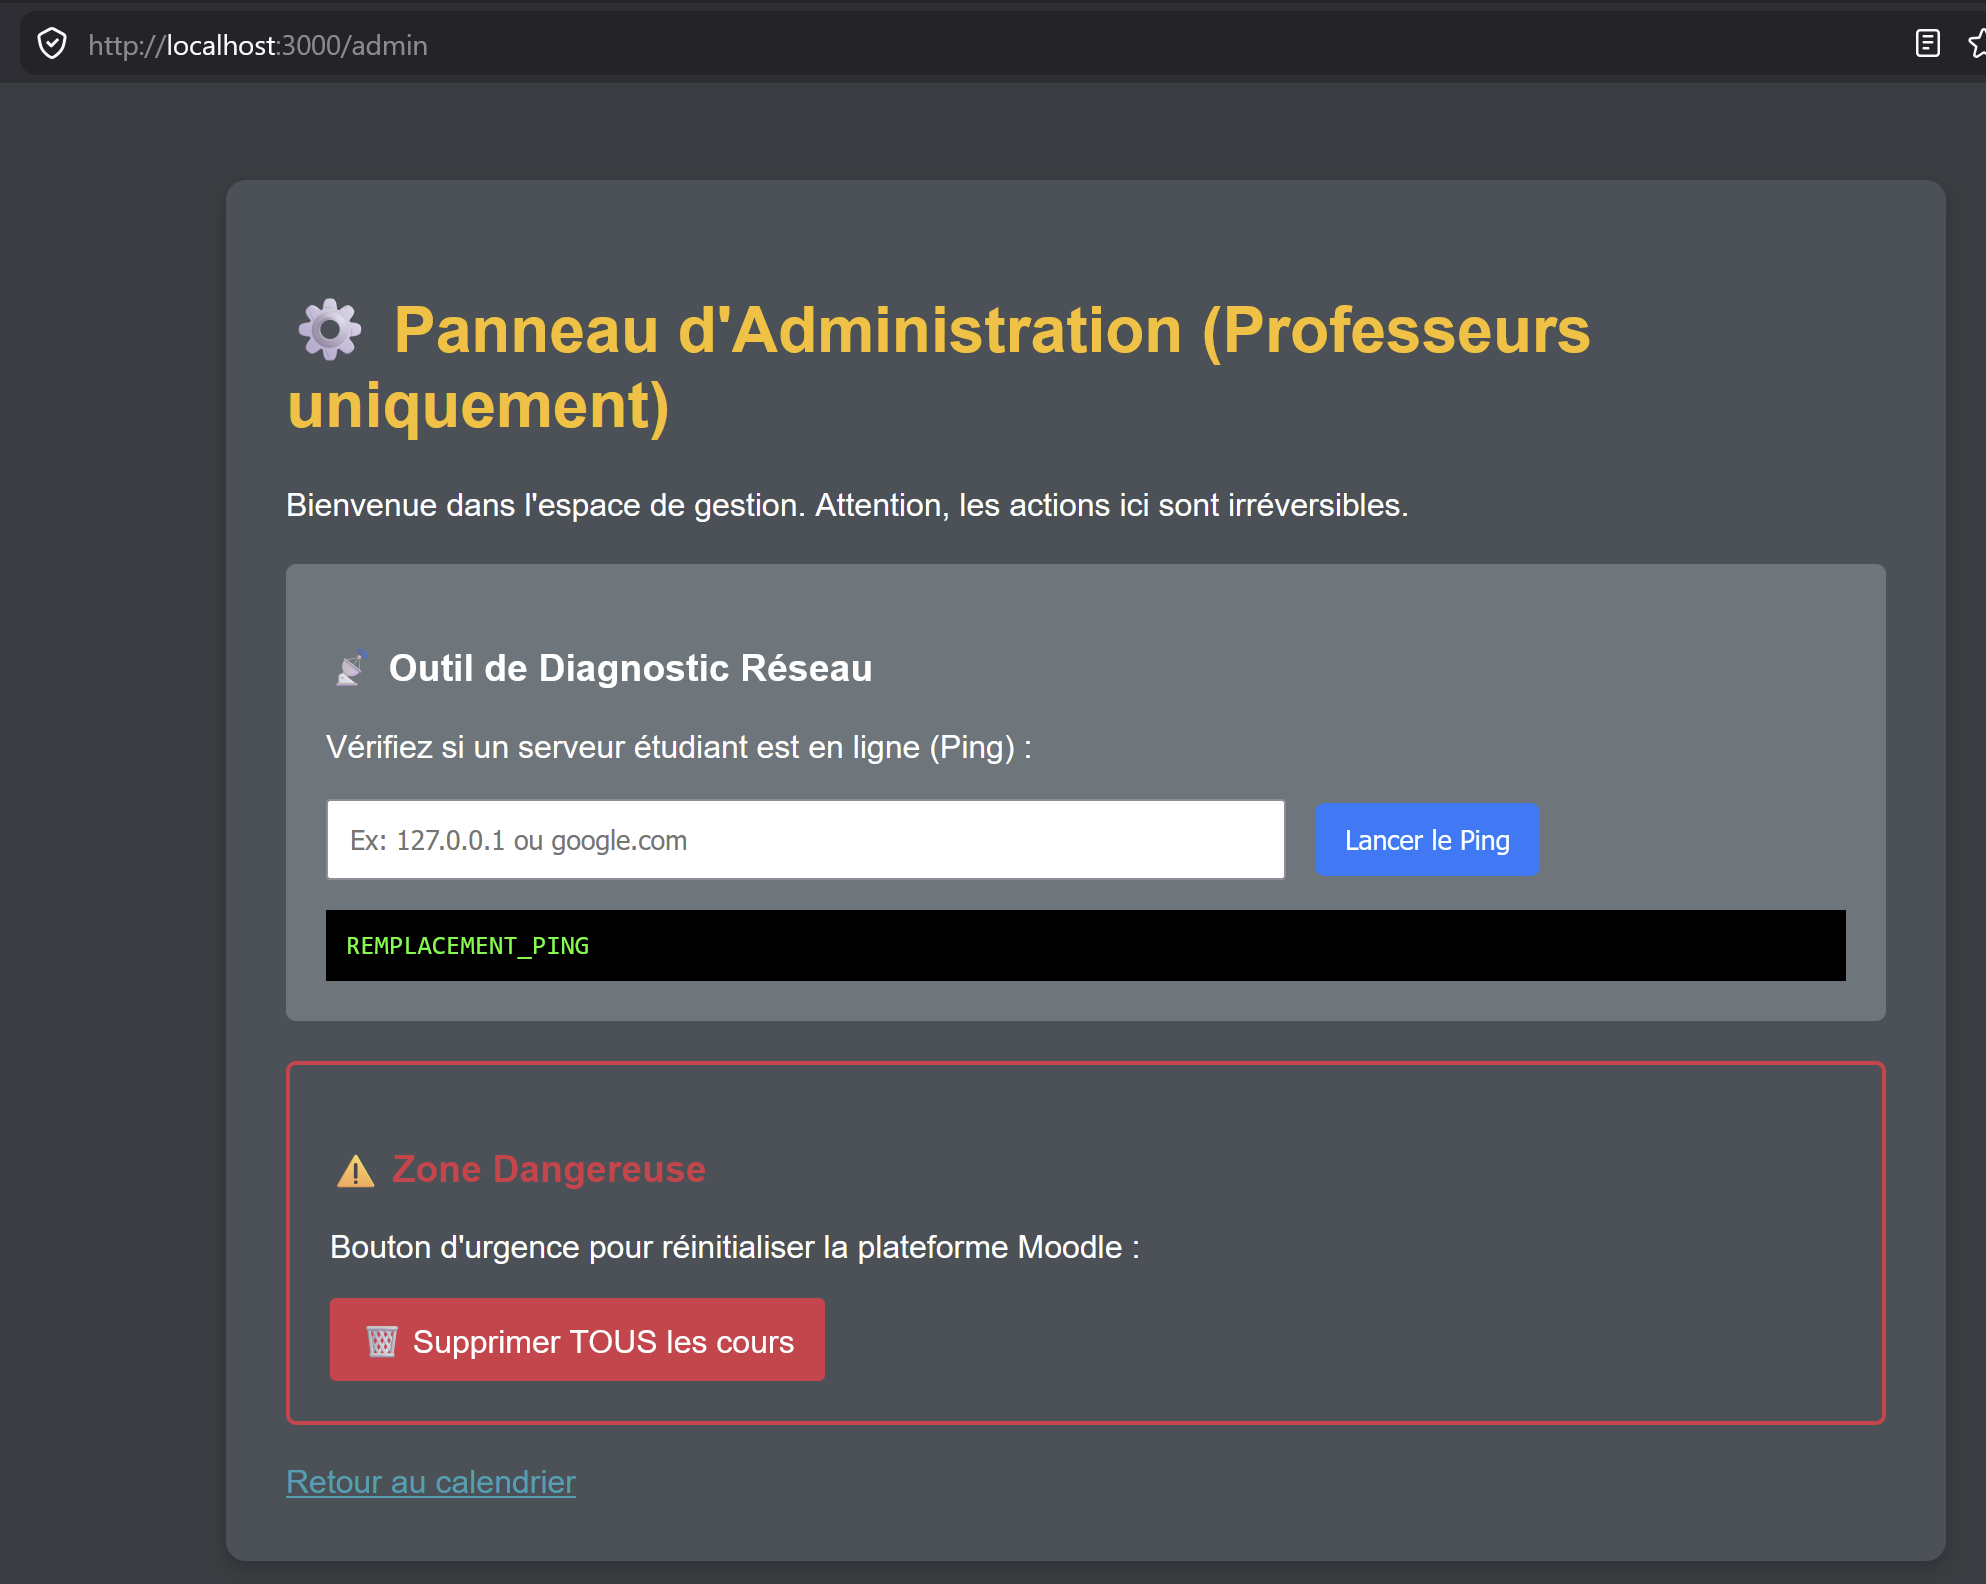
\includegraphics[width=0.8\linewidth]{pics/p6.png}
    \caption{Preuve de connexion à la page /admin}
    \label{fig:placeholder}
\end{figure}

\subsection{Impact}
Un attaquant ayant accès à cette page peut supprimer toutes les données de la plateforme, utiliser l'outil de diagnostic réseau et réaliser des actions irréversibles normalement réservées aux administrateurs.
\subsection{Recommandation}
 La correction consiste à vérifier côté serveur que l'utilisateur est connecté et possède le rôle admin avant d'afficher la page. Si ce n'est pas le cas, il doit être redirigé vers la page de connexion.
\newpage
% ══════════════════════════════════════════════════════════════════════════════
\section{Vulnérabilité 7 — Divulgation d'informations}

\subsection{Localisation}

Route \texttt{GET /debug/db}

\subsection{Description}
Une route de debug a été laissée accessible en production. En naviguant simplement vers /debug/db, n'importe qui peut accéder à l'intégralité de la base de données utilisateurs sans aucune authentification.

\subsection{Exploitation}
Accès direct via : http://localhost:3000/debug/db

\subsection{Preuve}

\begin{figure}[H]
    \centering
    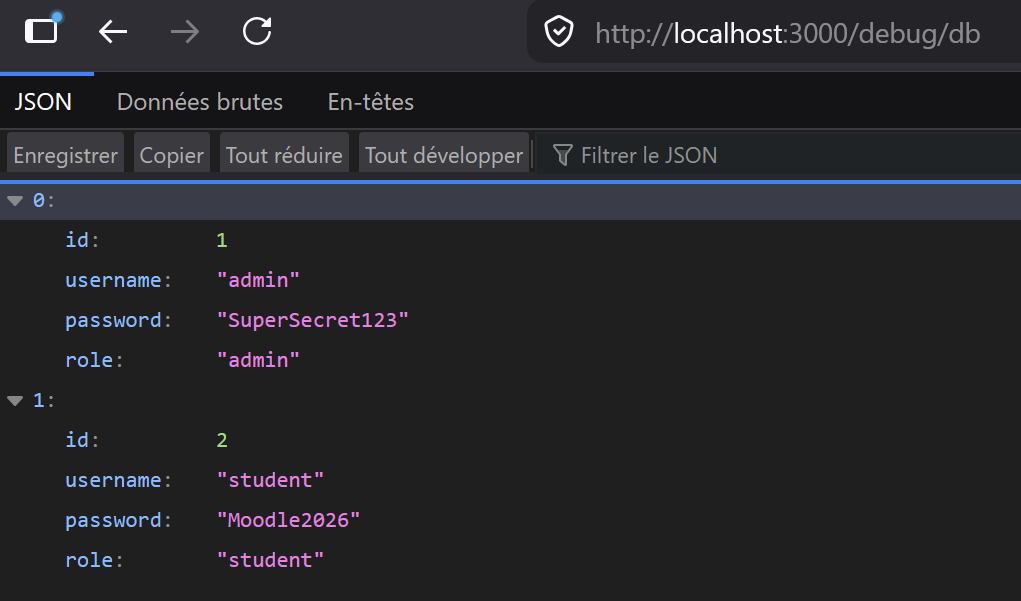
\includegraphics[width=0.8\linewidth]{pics/p7.png}
    \caption{Preuve de connexion à la BDD}
    \label{fig:placeholder}
\end{figure}

\subsection{Impact}
Tous les identifiants et mots de passe des utilisateurs sont exposés en clair. Un attaquant peut se connecter avec n'importe quel compte sans avoir besoin de casser quoi que ce soit.
\subsection{Recommandation}
 Supprimer toutes les routes de debug avant la mise en production. Les mots de passe doivent également être hashés et jamais stockés en clair.
\newpage
% ══════════════════════════════════════════════════════════════════════════════
\section{Conclusion}

Les vulnérabilités identifiées sont représentatives des erreurs les plus courantes en
développement web. 

\vspace{0.5cm}

Les corrections proposées sont simples à mettre en place et suffisantes pour éliminer ces vecteurs
d'attaque dans le cadre de ce projet.

\vspace{2cm}

\begin{flushright}
\textit{Romain LIGNERES — Red Team — ECE Paris 2025-2026}
\end{flushright}

\end{document}